\section{Estimativas, Cronogramas e Prazos}

\subsection{Estimativas}

\subsubsection{Dados Históricos Utilizados}
Não foram coletados dados históricos específicos para este tipo de projeto até o momento. As estimativas foram baseadas em:
\begin{itemize}
    \item Análise de complexidade de cada módulo
    \item Experiência da equipe em projetos similares
    \item Benchmarks da indústria para desenvolvimento web
    \item Consideração de integrações externas necessárias
    \item Metodologias ágeis de estimativa (Planning Poker)
\end{itemize}

\subsubsection{Técnicas de Estimativa Empregadas}
\begin{itemize}
    \item \textbf{Decomposição por Funcionalidades:} Divisão em módulos menores e estimativa individual
    \item \textbf{Análise de Pontos de Função:} Avaliação da complexidade baseada em entradas, saídas e processos
    \item \textbf{Estimativa por Analogia:} Comparação com sistemas similares já desenvolvidos
    \item \textbf{Consenso de Especialistas:} Validação das estimativas pela equipe técnica
    \item \textbf{Três Pontos:} Estimativa otimista, pessimista e mais provável para cálculo da média ponderada
\end{itemize}

\subsubsection{Estimativas por Sprint}
\begin{itemize}
    \item \textbf{Sprint 0 (Preparação):} 27 dias úteis - Documentação, análise e design
    \item \textbf{Sprint 1 (Desenvolvimento Inicial):} 26 dias úteis - Cadastros e funcionalidades básicas
    \item \textbf{Sprint 2 (Desenvolvimento Avançado):} 23 dias úteis - Sistema financeiro e cálculos
    \item \textbf{Sprint 3 (Finalização):} 10 dias úteis - Testes finais, correções e entrega
\end{itemize}

\textbf{Total do Projeto:} 86 dias úteis

\subsection{Cronograma}

\subsubsection{Estrutura de Trabalho}
Todo o trabalho será realizado em várias sprints de uma semana, organizadas em 4 ciclos principais, onde cada um desses ciclos contém diferentes números de sprints, respectivamente.

A organização das atividades e seu cronograma podem ser encontrados na tabela a seguir:

\subsubsection{Legenda}
\begin{itemize}
    \item \textbf{G} - Gerentes (Gestão e Planejamento)
    \item \textbf{A\&P} - Analistas e Programadores
    \item \textbf{COD} - Programadores (Codificação)
    \item \textbf{SQA} - Garantia da Qualidade (Testes)
\end{itemize}

\subsubsection{Cronograma Detalhado}

\begin{longtable}{|p{6cm}|c|c|c|c|}
\hline
\textbf{Atividade} & \textbf{Sprint 0} & \textbf{Sprint 1} & \textbf{Sprint 2} & \textbf{Sprint 3} \\
\hline
\multicolumn{5}{|c|}{\textbf{SPRINT 0 - PREPARAÇÃO (27 dias)}} \\
\hline
1.1 - Planejamento 0 (3d) - G & X & & & \\
\hline
1.2 - Criar Doc. Requisitos (10d) - A\&P & X & & & \\
\hline
1.2.1 - Revisar Doc. Requisitos (8d) - SQA & X & & & \\
\hline
1.3 - Doc. Casos de Uso (6d) - A\&P & X & & & \\
\hline
1.3.1 - Revisar Casos de Uso (2d) - SQA & X & & & \\
\hline
1.4 - Criar Modelo Conceitual (6d) - A\&P & X & & & \\
\hline
1.4.1 - Revisar Modelo Conceitual (3d) - SQA & X & & & \\
\hline
1.5 - Criar Diagrama Classes (4d) - A\&P & X & & & \\
\hline
1.5.1 - Revisar Diagrama Classes (2d) - SQA & X & & & \\
\hline
1.6 - Diagramas Sequência (5d) - A\&P & X & & & \\
\hline
1.6.1 - Revisar Diagramas Sequência (3d) - SQA & X & & & \\
\hline
\multicolumn{5}{|c|}{\textbf{SPRINT 1 - DESENVOLVIMENTO INICIAL (26 dias)}} \\
\hline
2.1 - Planejamento 1 (1d) - G & & X & & \\
\hline
2.1.1 - Criar Diag. Colaboração (3d) - A\&P & & X & & \\
\hline
2.1.2 - Revisar Diag. Colaboração (2d) - SQA & & X & & \\
\hline
2.1.3 - Integrar Diag. Colaboração (1d) - A\&P & & X & & \\
\hline
2.2 - Codificar Cadastro (13d) - COD & & X & & \\
\hline
2.3 - Testar Cadastro (5d) - SQA & & X & & \\
\hline
2.4 - Review (1d) - G & & X & & \\
\hline
\multicolumn{5}{|c|}{\textbf{SPRINT 2 - DESENVOLVIMENTO AVANÇADO (23 dias)}} \\
\hline
3.1 - Planejamento 2 (1d) - G & & & X & \\
\hline
3.2 - Codificar Despesas (14d) - COD & & & X & \\
\hline
3.3 - Testar Despesas (8d) - SQA & & & X & \\
\hline
\multicolumn{5}{|c|}{\textbf{SPRINT 3 - FINALIZAÇÃO (10 dias)}} \\
\hline
4.1 - Planning 3 (1d) - G & & & & X \\
\hline
4.2 - Corrigir Bugs (5d) - COD & & & & X \\
\hline
4.3 - Testes Finais (3d) - SQA & & & & X \\
\hline
4.4 - Preparar Entrega (1d) - G & & & & X \\
\hline
\end{longtable}

\subsection{Gráfico de Gantt}

O gráfico de Gantt completo do projeto está apresentado na figura abaixo, mostrando todas as atividades, suas dependências e alocação de recursos ao longo do tempo:

\begin{figure}[H]
    \centering
    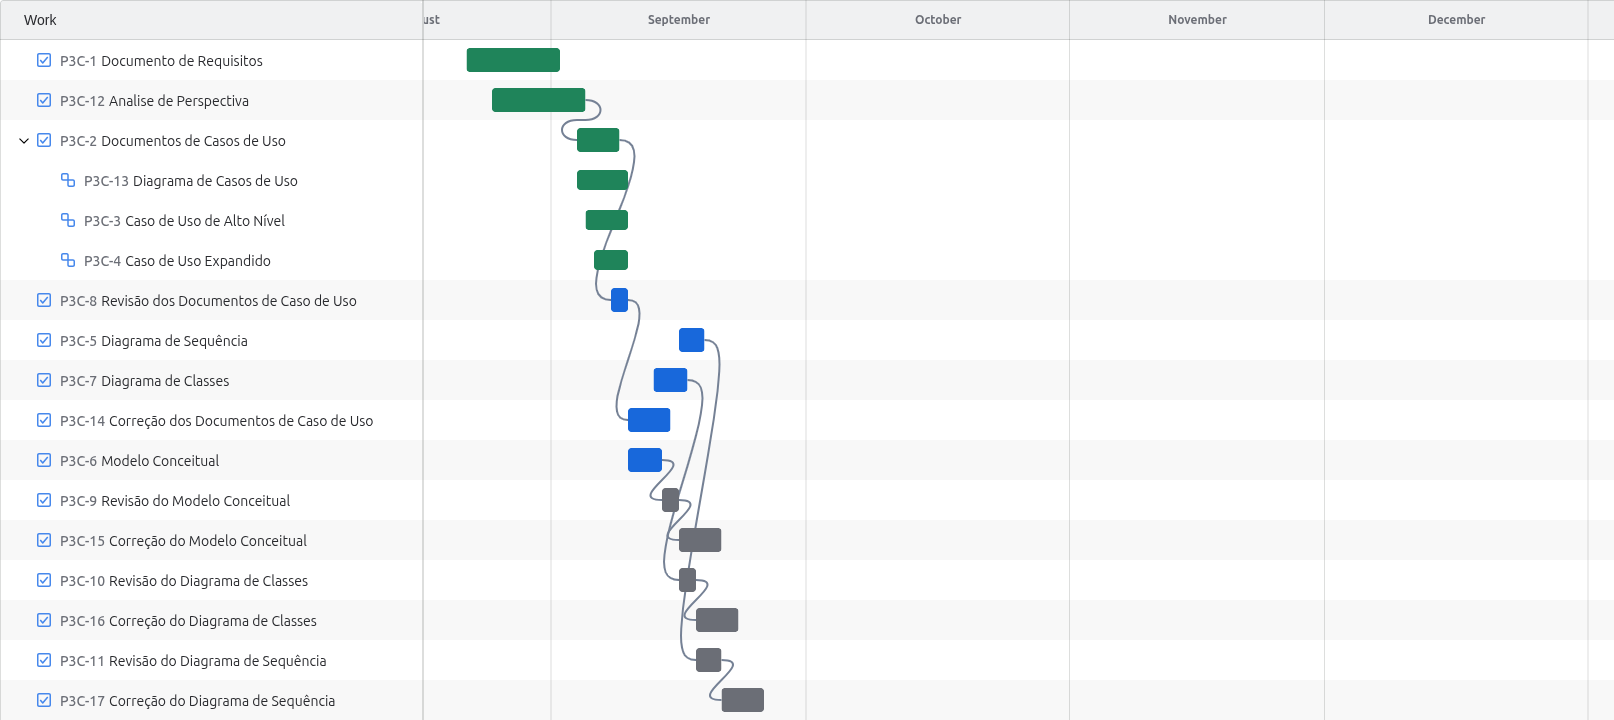
\includegraphics[width=\textwidth]{images/projeto_3___churrasco_2025-10-01_04.09pm.png}
    \caption{Gráfico de Gantt do Projeto - Sistema de Gestão de Churrascos Entre Amigos}
    \label{fig:gantt_chart}
\end{figure}

O gráfico de Gantt ilustra claramente:
\begin{itemize}
    \item A sequência temporal de todas as atividades
    \item As dependências críticas entre tarefas
    \item A alocação de recursos por equipe ao longo do tempo
    \item Os marcos principais de cada sprint
    \item O caminho crítico do projeto
\end{itemize}

\subsubsection{Caminho Crítico}
\textbf{Sequência do Caminho Crítico:} 1.1 → 1.2 → 1.3 → 1.4 → 2.1 → 2.1.1 → 2.1.2 → 2.1.3 → 2.2 → 2.3 → 2.4 → 3.1 → 3.2 → 3.3 → 4.1 → 4.2 → 4.3 → 4.4

Como o cronograma é totalmente sequencial, \textbf{todas as tarefas fazem parte do caminho crítico}. Qualquer atraso em uma tarefa atrasa o projeto inteiro.

\subsection{Marcos Principais}
\begin{itemize}
    \item \textbf{M0 (Fim do Sprint 0):} Documentação completa e aprovada - Dia 27
    \item \textbf{M1 (Fim do Sprint 1):} Módulo de cadastros funcionando - Dia 53
    \item \textbf{M2 (Fim do Sprint 2):} Sistema financeiro implementado - Dia 76
    \item \textbf{M3 (Fim do Sprint 3):} Sistema completo e entregue - Dia 86
\end{itemize}

\subsection{Entregáveis por Sprint}
\begin{itemize}
    \item \textbf{Sprint 0:} Documento de Requisitos, Casos de Uso, Diagramas UML
    \item \textbf{Sprint 1:} Módulo de cadastros funcionando, Diagramas de Colaboração
    \item \textbf{Sprint 2:} Sistema financeiro completo, Módulo de despesas
    \item \textbf{Sprint 3:} Sistema integrado, testado e documentado
\end{itemize}

\subsection{Critérios de Aceitação}
Cada marco deve atender aos seguintes critérios:
\begin{itemize}
    \item Todos os entregáveis foram revisados e aprovados pela equipe SQA
    \item Cobertura de testes mínima de 80\% para código
    \item Documentação atualizada e revisada
    \item Aprovação formal dos gerentes de projeto
\end{itemize}
